\section{Float Features: Figures, Tables etc.}
In \cref{fig:censorbox,tab:font_examples}, we have already seen examples for floats.
These are handled by packages \texttt{caption} and \texttt{floatrow}.
Notable features are the capability to have captions the same width as the float they are attached to.
This tends to look much prettier, \iecfeg{cf.} \cref{fig:wide_caption,fig:tighter_caption}.
%%%%%%%%%%%%%%%%%%%%%%%%%%%%%%%%%%%%%%%%%%%%%%%%%%%%%%%%%%%%%%%%%%%%%%%%%%%%%%%%%%%%%%%%%%%
\begin{figure}
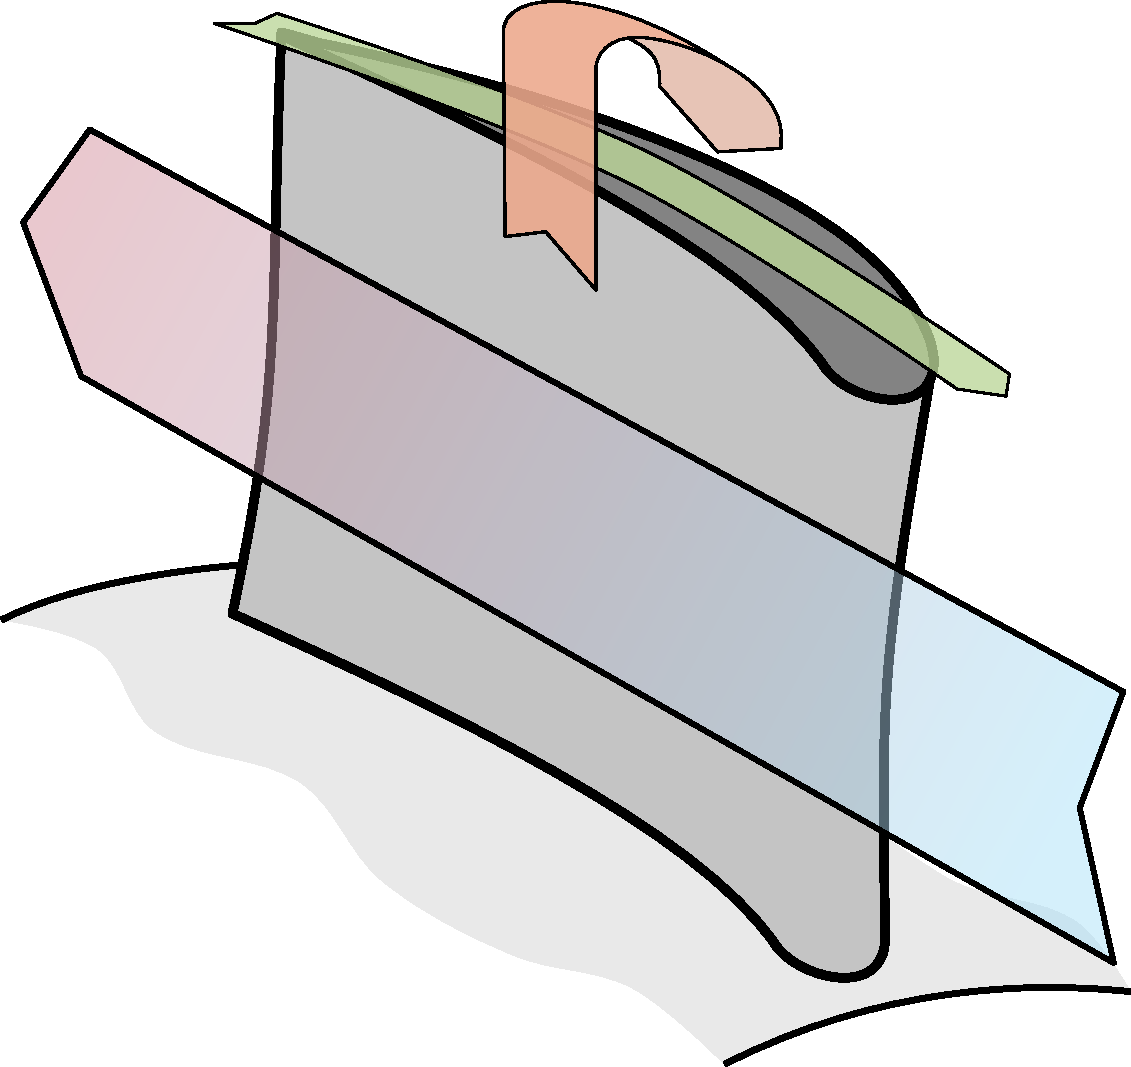
\includegraphics[width=0.4\textwidth]{example_image}%
\caption{Example for a regular caption, spanning the whole width since it is so long}%
\label{fig:wide_caption}%
\end{figure}
\begin{figure}
\ffigbox[\FBwidth]% Optional argument FBwidth causes graphic to be its actual size and caption to take up the remaining space. Otherwise, horizontal space is split 50/50, which doesn't make much sense.
{%
	\caption{Example for a new caption, spanning the just the width of the float it is attached to}%
	\label{fig:tighter_caption}%
}%
{%
	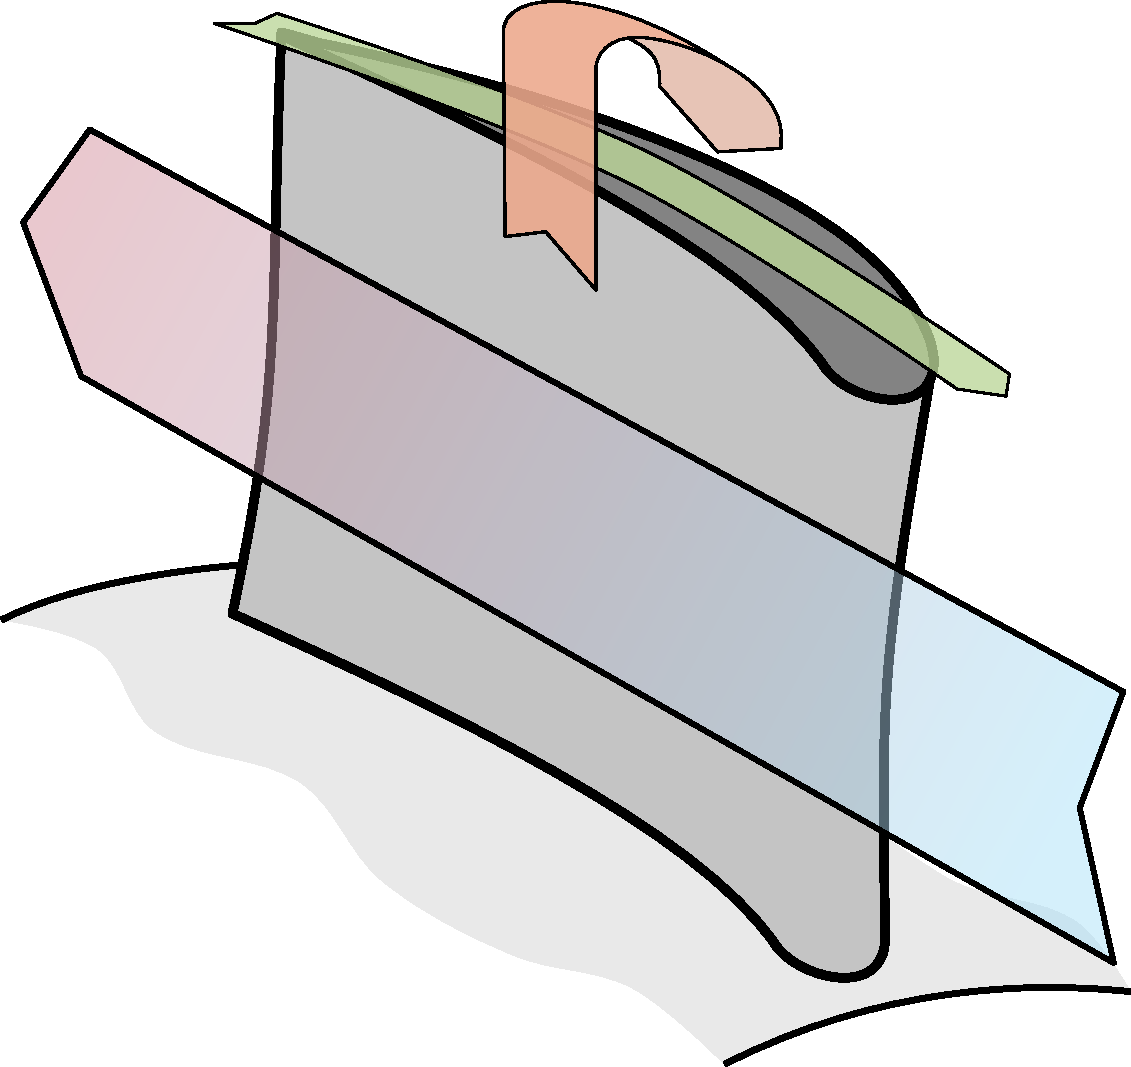
\includegraphics[width=0.4\textwidth]{example_image}%
}%
\end{figure}
%%%%%%%%%%%%%%%%%%%%%%%%%%%%%%%%%%%%%%%%%%%%%%%%%%%%%%%%%%%%%%%%%%%%%%%%%%%%%%%%%%%%%%%%%%%
\paragraph{Multiple floats}
Other possibilities are rather arbitrary arrangements of sub-figures and -captions.
For this, see \cref{fig:impeller_throat}, which contains two sub-figures \cref{fig:impeller_throat_iso,fig:impeller_throat_flat}.
Multiple sub-tables are also possible, see \cref{tab:works_on_turbocharging}.
\begin{figure}
\ffigbox[\FBwidth]
{%
	\begin{subfloatrow}[2]% Default is two anyway
		\ffigbox[\FBwidth]
		{%
			\def\svgwidth{0.4\figurewidth}
			\input{./images/impeller_isometric.pdf_tex}% input is not includegraphics, so we have to give the full path
		}%
		{%
			\caption{Isometric}%
			\label{fig:impeller_throat_iso}%
		}%
		\ffigbox[\FBwidth]
		{%
			\def\svgwidth{0.3\figurewidth}
			\input{./images/inducer_throat.pdf_tex}
		}%
		{%
			\caption{Schematic}%
			\label{fig:impeller_throat_flat}%
		}%
	\end{subfloatrow}
}%
{%
	\caption[Impeller Throat]%
	{%
		Inducer throat created by geometric constraints%
	}%
	\label{fig:impeller_throat}%
	\floatfoot{\adaptedfrom{} \autocites{shakal_centrifugal_2015}[99]{whitfield_design_1990}[535]{hayami_flow_1985}}%
}%
\end{figure}
\begin{table}
	\tiny
	\floatbox{table}%
	{%https://tex.stackexchange.com/q/295567/120853
		\begin{subfloatrow}
			\ttabbox[\FBwidth]%
			{%
				\begin{tabular}{@{}m{0.25\textwidth}m{0.15\textwidth}@{}}
					\toprule
					Author \& [Work] & Comment\\
					\midrule
					\textcite{bozza_map-based_2011} & ---\\
					\textcite{bozza_numerical_2013} & ---\\
					\textcite{bozza_theoretical_1990} & \textbf{Nozzles}\\
					\textcite{burke_modelling_2014} & ---\\
					\textcite{de_bellis_development_2018} & ---\\
					\textcite{berndt_einfluss_2009} & ---\\
					\textcite{chesse_performance_2000} & ---\\
					\textcite{cornolti_1d_2013} & ---\\
					\textcite{eriksson_modeling_2007} & ---\\
					\textcite{grigoriadis_experimentelle_2008} & ---\\
					\textcite{kech_model-based_2002} & ---\\
					\textcite{lee_simulation-based_2009} & ---\\
					\textcite{leufven_surge_2011} & ---\\
					\textcite{shaaban_part-load_2006} & ---\\
					\textcite{wahlstrom_modelling_2011} & ---\\
					\textcite{watel_matching_2010} & \mtlbsmlnk{}\\
					\textcite{yang_mixed_2010} & ---\\
					\bottomrule
				\end{tabular}
			}%
			{%
				\caption{Using Maps}%
				\label{tab:works_using_maps}%
			}%
			\ttabbox[\FBwidth]%
			{%
				\begin{tabular}{@{}m{0.25\textwidth}m{0.15\textwidth}@{}}
					\toprule
					Author \& [Work] & Comment\\
					\midrule
					\textcite{beckey_compressor_2011} & using algorithms\\
					\textcite{bergqvist_prediction_2014} & from CFD\\
					\textcite{bohn_modellierung_2002} & ---\\
					\textcite{bolz_critical_2014} & ---\\
					\textcite{elkamel_experimental_2011} & ---\\
					\textcite{ewert_modellierung_2013} & ---\\
					\textcite{freeman_compressor_2011} & \mtlb{} script\\
					\textcite{hansch_untersuchung_2010} & ---\\
					\textcite{harley_inlet_2014} & ---\\
					\textcite{luddecke_engine_2014} & ---\\
					\textcite{kurzke_correlations_2011} & ---\\
					\textcite{schwarz_considerations_2014} & ---\\
					\bottomrule
				\end{tabular}
			}%
			{%
				\caption{Computing Maps}%
				\label{tab:works_computing_maps}%
			}%
		\end{subfloatrow}
		
		\begin{subfloatrow}
			\ttabbox[\FBwidth]%
			{%
				\begin{tabular}{@{}m{0.25\textwidth}m{0.15\textwidth}@{}}
					\toprule
					Author \& [Work] & Comment\\
					\midrule
					\textcite{aungier_mean_1995} & ---\\
					\textcite{casey_method_2013} & Calibrating with Maps\\
					\textcite{chen_one-dimensional_2014} & Turbine\\
					\textcite{erickson_centrifugal_2008} & \fortran{}\\
					\textcite{ewert_modellierung_2013} & ---\\
					\textcite{gong_total_2014} & ---\\
					\textcite{gutierrez_velasquez_one_2010} & \fortran{}, 1D and 3D\\
					\textcite{japikse_turbomachinery_2009} & Overview\\
					\textcite{kamaleshaiah_improved_1988} & ---\\
					\textcite{kessel_modellbildung_2002} & 1- \& 3D\\
					\textcite{lee_dual-stage_2008} & dual-stage; \textbf{\smlnk{}, maps}\\
					\textcite{nakhjiri_vatl_2018} & ---\\
					\textcite{okhuahesogie_1-d_2014} & Differential Evolution\\
					\textcite{pelton_one-dimensional_2007} & ---\\
					\textcite{pixberg_modellbildung_2013} & \textbf{Reservoirs; Nozzles} (p.\ 42)\\
					\textcite{sakellaridis_development_2015} & ---\\
					\textcite{schiffmann_design_2010} & ---\\
					\textcite{schlador_erstellung_2008} & \fortran{}, \textbf{Reservoirs; Models}\\
					\textcite{schur_transient_2013} & \smlnk{}\\
					\textcite{serrano_model_2008} & \textbf{Reservoirs; Nozzles}\\
					\textcite{shaaban_experimental_2004} & Diabatic; Extrapolation\\
					\textcite{stuart_analysis_2014} & cites \autocite{harley_evaluation_2013}\\
					\textcite{taburri_model-based_2012} & \textbf{Reservoirs; Nozzles}\\
					\textcite{uchida_transient_2006} & ---\\
					\textcite{whitfield_preliminary_1990} & Preliminary Design\\
					\textcite{wirz_berechnungsmethode_2017} & \textbf{Reservoirs; Models}\\
					\textcite{xu_empirical_2012} & ---\\
					\textcite{zahn_arbeitsspielaufgeloste_2012} & ---\\
					\textcite{zhuge_development_2009} & ---\\
					\bottomrule
				\end{tabular}
			}%
			{%
				\caption{Physical (0- \& 1D)}%
				\label{tab:works_physical}%
			}%
			\ttabbox[\FBwidth]%
			{%
				\begin{tabular}{@{}m{0.25\textwidth}m{0.15\textwidth}@{}}
					\toprule
					Author \& [Work] & Comment\\
					\midrule
					\textcite{aungier_mean_1995} & ---\\
					\textcite{doustmohammadi_experimental_2013} & ---\\
					\textcite{el-maksoud_prediction_2012} & ---\\
					\textcites{galvas_analytical_1972}{galvas_fortran_1973} & ---\\
					\textcite{gulich_disk_2003} & Disk Friction\\
					\textcite{gutierrez_velasquez_determination_2017} & ---\\
					\textcite{harley_evaluation_2013} & Recommends \autocite{oh_optimum_1997} \\
					\textcite{mohtar_increasing_2010} & ---\\
					\textcite{nakhjiri_physical_2011} & ---\\
					\textcite{oh_optimum_1997} & ---\\
					\textcite{tacconi_investigation_2018} & Cites \autocite{harley_evaluation_2013}; recommends \autocite{galvas_fortran_1973}\\
					\textcite{schneider_analytical_2015} & 2D\\
					\textcite{solaesa_analytical_2016} & ---\\
					\bottomrule
				\end{tabular}
			}%
			{%
				\caption{Loss Modelling}%
				\label{tab:works_losses}%
			}%
		\end{subfloatrow}%
	}%
	{%
		\caption[Works on zero- and one-dimensional modelling]
		{%
			Works on zero- and one-dimensional turbocharger and engine modelling%
		}%
		\label{tab:works_on_turbocharging}%
	}%
\end{table}
%%%%%%%%%%%%%%%%%%%%%%%%%%%%%%%%%%%%%%%%%%%%%%%%%%%%%%%%%%%%%%%%%%%%%%%%%%%%%%%%%%%%%%%%%%%
\paragraph{Side Captions}
Lastly, on occasion figures and their captions might look disproportionate in combination.
In these cases, placing a side-caption might relieve the situation, as shown in \cref{fig:sidecap}.
\begin{figure}
\fcapside[\FBwidth]%
{%
	\caption{A side caption, which may also span multiple lines like demonstrated in this rather long caption right here}
	\label{fig:sidecap}%
}%
{%
	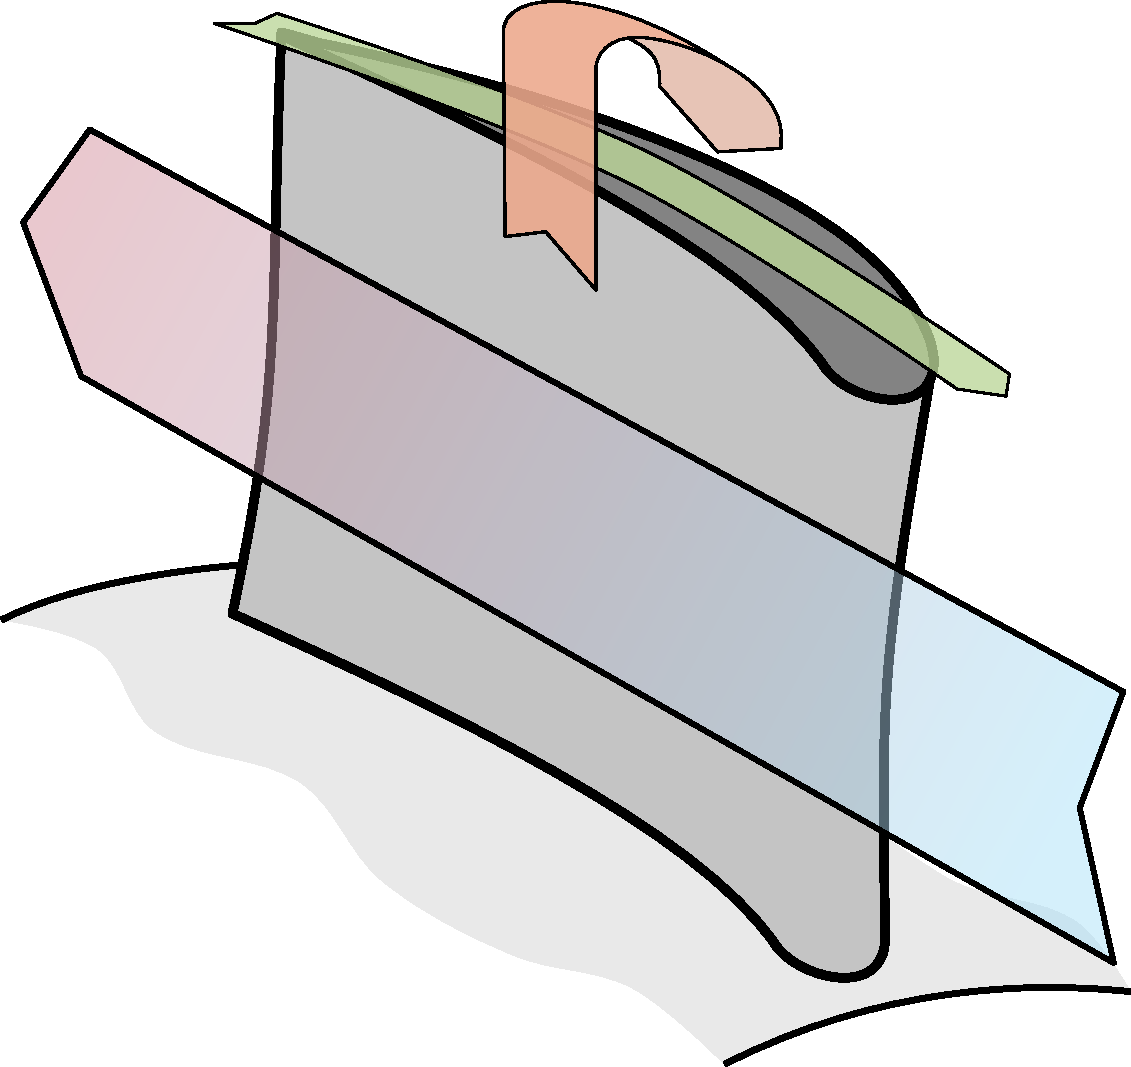
\includegraphics[width=0.4\textwidth]{example_image}%
}%
\end{figure}
%%%%%%%%%%%%%%%%%%%%%%%%%%%%%%%%%%%%%%%%%%%%%%%%%%%%%%%%%%%%%%%%%%%%%%%%%%%%%%%%%%%%%%%%%%%
\paragraph{Caption Position}
Note that the caption of \cref{tab:font_examples} occurs \textit{above} the table no matter the \texttt{caption} command's position.
Per convention, figure captions should appear below, table captions above their bodies.
This is also handled by \texttt{floatrow}.
Also note that there is neither a fullstop nor \textit{any} character (no space, no empty line) behind the last caption line in the source code, since dots are managed globally by the \texttt{caption} package.
\paragraph{Float Footer}
We also have a \verb|\floatfoot| command for all floats.
This is used to place additional info underneath the caption, primarily used for references.
%%%%%%%%%%%%%%%%%%%%%%%%%%%%%%%%%%%%%%%%%%%%%%%%%%%%%%%%%%%%%%%%%%%%%%%%%%%%%%%%%%%%%%%%%%%
%%%%%%%%%%%%%%%%%%%%%%%%%%%%%%%%%%%%%%%%%%%%%%%%%%%%%%%%%%%%%%%%%%%%%%%%%%%%%%%%%%%%%%%%%%%
\subsection{Tikz and pgfplots}
Packages \texttt{tikz} and \texttt{pgfplots} offer an absolutely scary plethora of features.
A select few are presented here%
\footnote{%
	By the way, footnotes look like this.%
}.
%%%%%%%%%%%%%%%%%%%%%%%%%%%%%%%%%%%%%%%%%%%%%%%%%%%%%%%%%%%%%%%%%%%%%%%%%%%%%%%%%%%%%%%%%%%
\paragraph{Drawing over Bitmaps}
When having to rely on bitmaps, once might still want to add additional info.
This can be done directly in \LaTeX{}, profiting from all the usual features.
In the example here, this is of course the retaining of the text font, but also usage of the wonderful \texttt{contour} package to draw legible black-on-white (or vice-versa) text.
An example is shown in \cref{fig:mtu_turbo}.
\begin{figure}
\ffigbox[\FBwidth]
{%
	\begin{tikzpicture}% https://tex.stackexchange.com/a/9562/120853
	[every path/.style = {draw, line width = 5pt, rounded corners, white},
	font = \sffamily,
	]
	\node[anchor=south west,inner sep=0] (img) at (0,0) {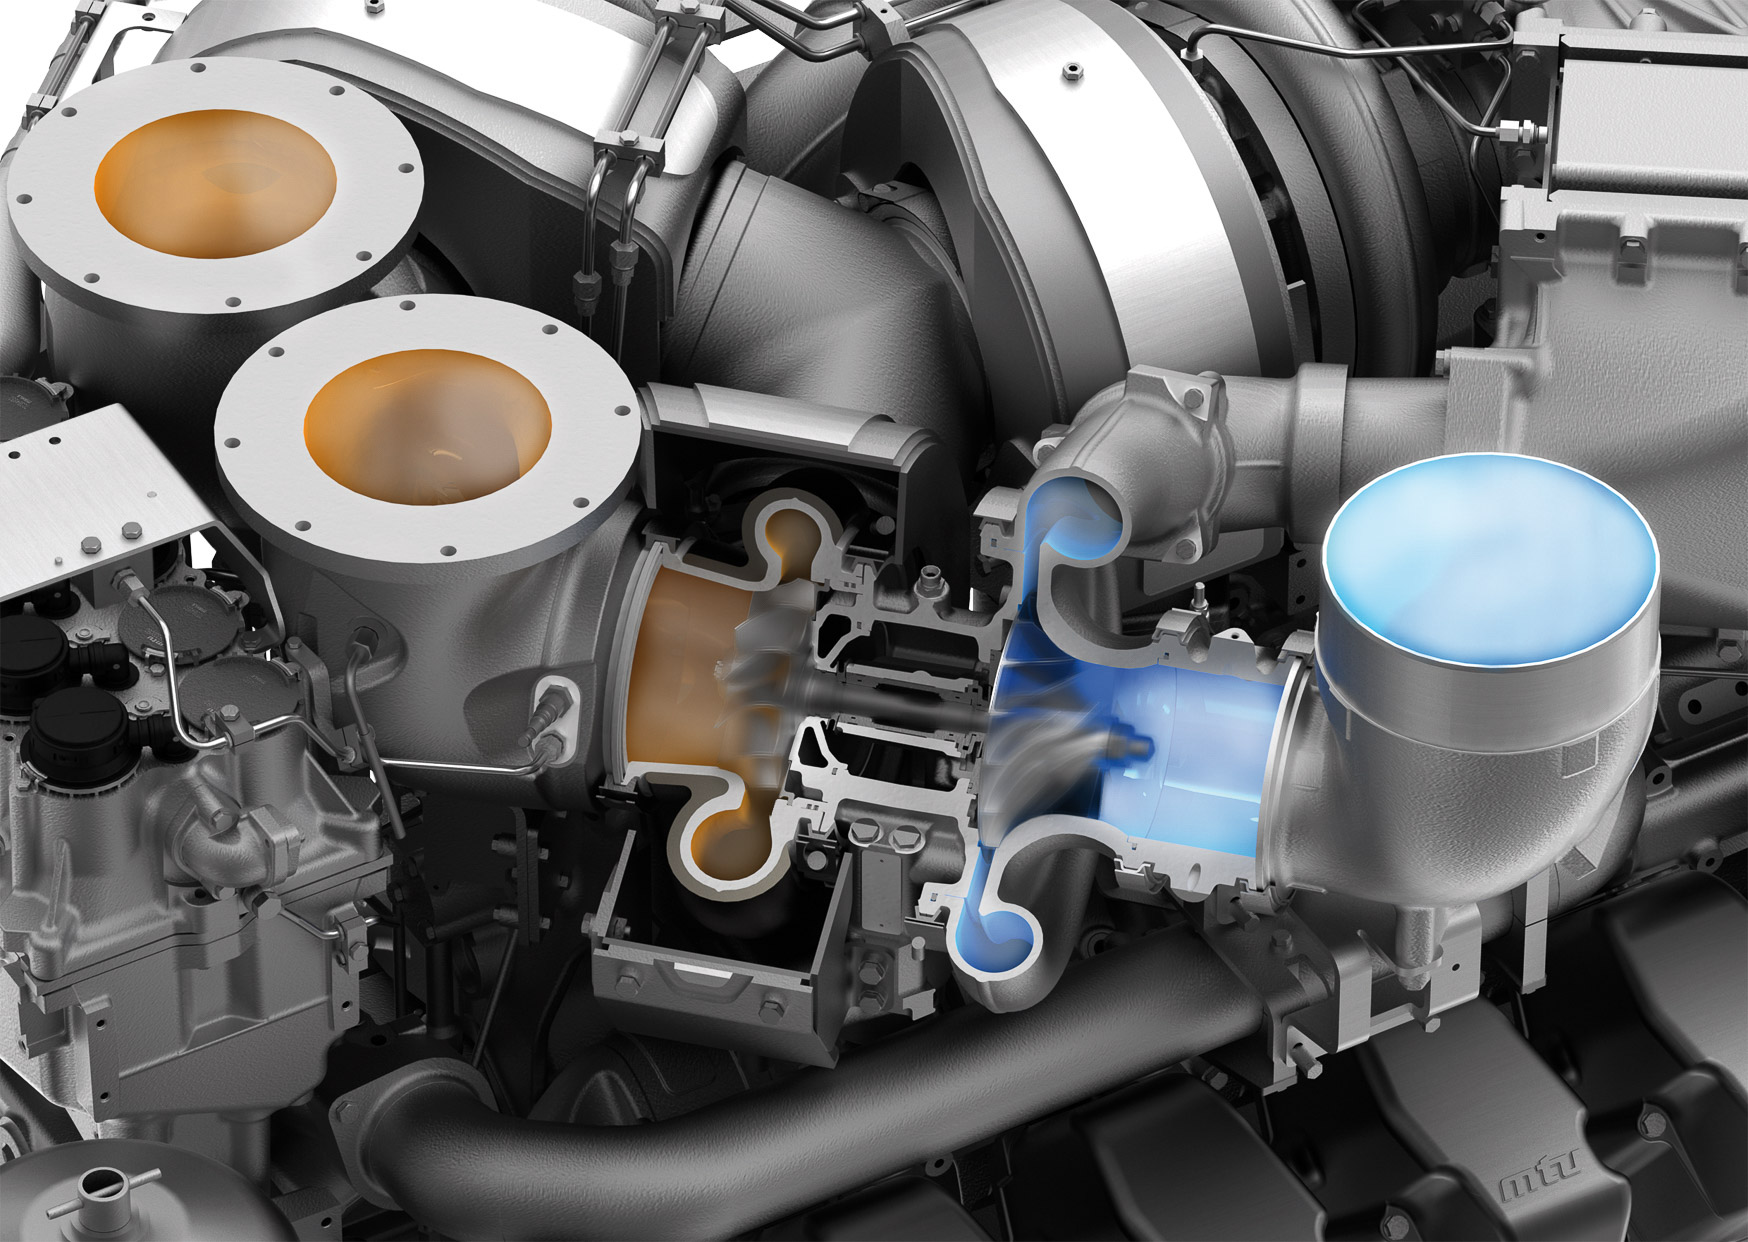
\includegraphics[width=0.7\textwidth]{mtu_turbo.jpg}};
	\begin{scope}[x={(img.south east)}, y={(img.north west)}]

	% Air Intake in the right:
	\node at (0.85, 0.55) {\ctrb{Air In}};

	% Turbine:
	\node[outer sep = 10pt] (turbine) at (0.45, 0.45) {};
	\node[below left = of turbine] (turbinetext) {\ctrb{Turbine Wheel}};
	\draw[-stealth] (turbinetext) to[out = 0, in = -120] (turbine);

	% Shaft:
	\node[outer sep = 5pt] (shaft) at (0.525, 0.43) {};
	\node[above = of shaft] (shafttext) {\ctrb{Shaft}};
	\draw[-stealth] (shafttext) to (shaft);

	% Compressor:
	\node[outer sep = 10pt] (compressor) at (0.6, 0.4) {};
	\node[below right = of compressor] (compressortext) {\ctrb{Impeller}};
	\draw[-stealth] (compressortext) to[out = 180, in = -45] (compressor);

	%\draw[help lines,xstep=.1,ystep=.1] (0,0) grid (1,1);% Uncomment block for coordinate help lines
	%	\foreach \x in {0,1,...,9} { \node [anchor=north] at (\x/10,0) {0.\x};}
	%	\foreach \y in {0,1,...,9} { \node [anchor=east] at (0,\y/10) {0.\y};}
	\end{scope}
	\end{tikzpicture}
}%
{%
	\caption[Turbocharger Rendering]%
	{
		Digital rendering of a \emph{Rolls-Royce Power Systems/MTU} turbocharger unit.
		Note the two-stage (arrangement in series) setup%
	}
	\label{fig:mtu_turbo}
	\floatfoot{\adaptedfrom{} \autocite{rolls-royce_power_systems_ag_mtu_2011}}
}
\end{figure}
%%%%%%%%%%%%%%%%%%%%%%%%%%%%%%%%%%%%%%%%%%%%%%%%%%%%%%%%%%%%%%%%%%%%%%%%%%%%%%%%%%%%%%%%%%%
\paragraph{Direct plotting}
If you rely on tools like \texttt{matlab2tikz}, maybe this is for you.
We can plot \textit{directly} into \LaTeX, without having to import outside data in the form of \texttt{*.csv}-files or automatically generated Tikz-pictures.
Still, anything more than polynomials is probably still too much.
While the functionality is limited, it may still save a lot of time and headaches.
This is demonstrated in \cref{fig:plotting_in_latex,fig:plotting_in_latex_tufte}.
\begin{figure}\ContinuedFloat*% We can continue floats across pages like this
\fcapside[\FBwidth]
{%
\caption{
	Caloric parameters of air.
	Avoid legends and put info where it belongs, improving legibility (less back-and-forth for the eye)%
	}%
\label{fig:plotting_in_latex}%
\floatfoot{See \autocite[15]{dixon_fluid_2014}}%
}%
{%
\begin{tikzpicture}
	\begin{axis}[%
	plotstyleNarrow,%
	axis y line*=right,%
	axis x line=none,%
	grid=none,
	ylabel={\gls{adexp}},% Using \ensuremath{} for each symbol, we don't have to use math mode here
	y unit = {-},
	]
		\addplot+[domain=20:400]{cpm(x)/(cpm(x)-8.3145)} node [pos=0.3, fill=white, inner sep=0.5pt, sloped] {\gls{adexp}};
	\end{axis}
	\begin{axis}[% https://tex.stackexchange.com/a/31504/120853
	plotstyleNarrow,%
	xlabel={\gls{c_temperature}},%
	x unit = {\degreeCelsius},
	ylabel={\gls{specheatcappres}},
	y unit = {\joule\per\kilogram\per\kelvin},
	cycle list shift=1,
	]
		\addplot+[domain=20:400]{cpm(x)/0.0289524} node [pos=0.3, fill=white, inner sep=0.5pt, sloped] {\gls{specheatcappres}};%
	\end{axis}
\end{tikzpicture}
}%
\end{figure}

\begin{figure}\ContinuedFloat
\fcapside[\FBwidth]
{%
	\caption{Same as \cref{fig:plotting_in_latex} in hip and \enquote{\textit{Tufte}-like}}
	\label{fig:plotting_in_latex_tufte}
}%
{%
\begin{tikzpicture}
	\begin{axis}[%
	minimalistic,%
	ylabel={\gls{specheatcappres}},
	y unit = {\joule\per\kilogram\per\kelvin},
	xlabel={\gls{temperature}},%
	x unit = {\kelvin},
	domain=300:700,
	ymin = 1000,
	ymax = 1100,
	ytick = {1000, 1050, 1100},% Specify manually due to weird rounding
	]
		\addplot+{cpm(x-273.15)/0.0289524} node [pos = 0.3,fill=white,inner sep=0.5pt, sloped] {\gls{specheatcappres}};%
	\end{axis}%
	\begin{axis}[% https://tex.stackexchange.com/a/31504/120853
	minimalistic,%
	axis y line*=right,%
	axis x line=none,%
	ylabel={\gls{adexp}},%
	y unit = {-},
	cycle list shift=1,
	domain = 300:700,
	ymin = 1.35,
	ymax = 1.4,
	]
		\addplot+{cpm(x-273.15)/(cpm(x-273.15)-8.3145)} node [pos = 0.3,fill=white,inner sep=0.5pt, sloped] {\gls{adexp}};
	\end{axis}
\end{tikzpicture}
}%
\end{figure}
%%%%%%%%%%%%%%%%%%%%%%%%%%%%%%%%%%%%%%%%%%%%%%%%%%%%%%%%%%%%%%%%%%%%%%%%%%%%%%%%%%%%%%%%%%%
\paragraph{From a file}
As discussed, often we'd want to plot data from files.
The better behaved the CSV file is (meaningful headers, no junk rows), the easier that is.
In \cref{fig:diffuser}, we only have to specify \iecfeg{e.g.} \verb|y=M| and the column corresponding to that header is automatically chosen, with no confusion about indices/numbers.
\begin{figure}
\ffigbox[\FBwidth]
{
	\caption{A plot from CSV data for a diffuser}
	\label{fig:diffuser}
}%
{%
\pgfplotstableread{./data/diffuser.csv}{\diffusertable}%
\begin{tikzpicture}
	\begin{axis}%
	[%
	minimalistic,%
	axis y line*=left,%
	xlabel={\(\gls{radius}/\gls{radius}_{2}\)},%
	x unit = {-},
	ylabel={\gls{mach}, \(\gls{pressure}/\gls{pressure}_{2}\), \(\gls{temperature}/\gls{temperature}_{2}\), \(\gls{density}/\gls{density}_{2}\)},%
	y unit = {-},
	table/x={R_pres},%
	ymin=0.4,
	ymax=1.3,
	ytick={0.4, 0.7, 1, 1.3},
	xmin=1,
	xmax=1.6
	]%
		% Do this manually, node macro expansion in foreach/invokeforeach is weird
		\addplot+ table [y=M] {\diffusertable} node [pos=0.2, fill=white] {\gls{mach}};
		\addplot+ table [y=Pi] {\diffusertable} node [pos=0.9, fill=white] {\(\gls{pressure}/\gls{pressure}_{2}\)};
		\addplot+ table [y=Theta] {\diffusertable} node [pos=0.7, fill=white] {\(\gls{temperature}/\gls{temperature}_{2}\)};
		\addplot+ table [y=Rho] {\diffusertable} node [pos=0.8, fill=white] {\(\gls{density}/\gls{density}_{2}\)};
	\end{axis}%
	\begin{axis}%
	[%
	minimalistic,%
	axis y line*=right,%
	axis x line=none,%
	ylabel = {abs.\ flow angle \gls{angabs}},%
	y unit = {\degree},
	cycle list shift=4,%
	ymin=13,
	ymax=15,
	xmin=1,
	xmax=1.6,
	]%
		\addplot+ table [x=R_pres, y=alpha] {\diffusertable} node [pos=0.6, fill=white] {\gls{angabs}};%
	\end{axis}%
\end{tikzpicture}
}
\end{figure}
%%%%%%%%%%%%%%%%%%%%%%%%%%%%%%%%%%%%%%%%%%%%%%%%%%%%%%%%%%%%%%%%%%%%%%%%%%%%%%%%%%%%%%%%%%%
\paragraph{Tikz and Text}
We can also draw tikz content into text content using \texttt{tikzmark}.
This, and also how to use \verb|\foreach| in tikz, is illustrated in \cref{eq:tikz_in_text}.
There, usage of chemical compounds as \verb|\chcpd| is also shown.

\noindent%
\begin{minipage}{1\linewidth}
\medmuskip = 3\medmuskip% https://tex.stackexchange.com/q/83746/120853
\thickmuskip = 3\thickmuskip
{%
\begin{equation}\label{eq:tikz_in_text}
\tikzmark{c}\gls{massfr}_{\chcpd{C}} + \tikzmark{h}\gls{massfr}_{\chcpd{H}} + \tikzmark{s}\gls{massfr}_{\chcpd{S}} + \tikzmark{o}\gls{massfr}_{\chcpd{O}} + \tikzmark{n}\gls{massfr}_{\chcpd{N}} + \tikzmark{w}\gls{massfr}_{\chcpd{H2O}} + \tikzmark{a}\gls{massfr}_{\mathrm{ash}}\coloneq 1\eqend{}
\end{equation}
\begin{tikzpicture}[remember picture,overlay]
\pgfmathsetmacro{\vshiftone}{4}
\pgfmathsetmacro{\vshifttwo}{6.5}
\pgfmathsetmacro{\vshiftthree}{9}
\pgfmathsetmacro{\hshiftone}{1}
\pgfmathsetmacro{\hshifttwo}{2}
\pgfmathsetmacro{\hshiftthree}{3}

\foreach \x/\y/\a/\b in {%
	c/Carbon/\vshiftone/-\hshiftthree,%
	h/Hydrogen/\vshifttwo/-\hshifttwo,%
	s/Sulphur/\vshiftthree/-\hshiftone,%
	o/Oxygen/\vshifttwo/0,%
	n/Nitrogen/\vshiftthree/\hshiftone,%
	w/Water/\vshifttwo/\hshifttwo,%
	a/Ash/\vshiftone/\hshiftthree%
}%
{%
	\node (\x1) [below right = 0.1em and 0.4em of pic cs:\x] {};
	\node (\x2) [on grid, below right = \a ex and \b ex of \x1, anchor=north] {\y};% On grid makes positioning snappy (uses actual middle of nodes); without, even 'right=0pt' would not be centered
	\draw[-stealth] [out=90] (\x2) to [in=270](\x1);
}%
\end{tikzpicture}
}%
\vspace{11ex}% We need to use 'overlay', but this also means we lose the bounding box. Eye-ball it here, sadly.
\end{minipage}

%%%%%%%%%%%%%%%%%%%%%%%%%%%%%%%%%%%%%%%%%%%%%%%%%%%%%%%%%%%%%%%%%%%%%%%%%%%%%%%%%%%%%%%%%%%
\paragraph{Regular Tikz pictures}
Tikz really is \textit{not} meant for drawing.
The more free-form images shown here were created in InkScape.
Still, \enquote{quoting} in Tikz is much preferred and nicer when the images are somewhat programmatic, aka there's a lot of \SI{90}{\degree} corners, equal distances, and everything is a bit \enquote{block-like}.
Then, your chances of success using Tikz are much improved, for it is suited well then.
For example, a small file structure diagram:

\begin{tikzpicture}[%http://www.texample.net/tikz/examples/filesystem-tree/
grow via three points={one child at (0.5,-0.7) and
	two children at (0.5,-0.7) and (0.5,-1.4)},
edge from parent path={(\tikzparentnode.south) |- (\tikzchildnode.west)},
every node/.style={draw=black,thick,anchor=west,fill=g5},
font=\ttfamily,%
]%
\node {\faFileO{} parent.py}
child { node {\faFileO{} constants.py}}
child { node {\faFileO{} parameters.py}}
child { node {\faFileO{} handling.py}}
child { node {\faFileO{} performance\_maps.py}};
\end{tikzpicture}

Note how \texttt{tikzpicture} environments don't have to be contained in floats.
A second example is shown in \cref{fig:tikz_diagram}.

\begin{figure}
\ffigbox[0.95\linewidth]
{%
	\begin{tikzpicture}%https://tex.stackexchange.com/a/166254/120853
	[%
	every path/.style={thick},%https://tex.stackexchange.com/a/302931/120853
	]%
	
	% Row of Model Blocks
	\node[simblock, minimum height = 5ex] (outlet) {Outlet};
	\node[simblock, minimum height = 5ex, right = of outlet] (turbine) {Turbine};
	\node[simblock, minimum height = 5ex, right = of turbine] (compressor) {Compressor};
	\node[simblock, minimum height = 5ex, right = of compressor] (inlet) {Inlet};
	\draw[->] (outlet) -- (turbine) node [midway, above, font = \footnotesize] {feeds};
	\draw[->] (turbine) -- (compressor) node [midway, above, font = \footnotesize, align = center] (shaft) {via\\shaft};
	\draw[->] (compressor) -- (inlet) node [midway, above, font = \footnotesize] {feeds};
	
	% Division Block underneath Engine
	\node[below = 12ex of inlet.south, draw= none] (div) {};
	\node[below = 4ex of div, draw = none] (mult) {};
	\node[simblock, fit = (mult) (div), minimum height = 8ex] (multdiv) {};
	\node at (div) {\(\div\)};
	\node at (mult) {\(\ast\)};
	
	% Connect Inlet and Division part
	\draw[->] (inlet.east) -- ++ (+1, 0)  node [pos=1, above] {\(p\mr{\gls{inlet}}(\tau)\)} |- ($(multdiv.east)!0.5!(multdiv.north east)$);
	
	% p min block next to multiplication
	\draw[<-] ($(multdiv.east)!0.5!(multdiv.south east)$) -- ++ (1, 0) node[simblock] {\(p\mr{\gls{air},\gls{ratedeng}}\)};
	
	\node [circle, fill, inner sep = 0.3ex, left = 0.7em of multdiv] (split1) {};
	\draw (multdiv) -- (split1);
	
	% Bias and inverted Bias blocks
	\node[simblock, left = of div] (biasinv) {\(1 - u\)};
	\node[simblock, left = of mult] (bias) {\(u - 1\)};
	\draw[->] (split1) |- (bias);
	\draw[->] (split1) |- (biasinv);
	
	% Split again
	\node [circle, fill, inner sep = 0.3ex, left = 1em of biasinv] (split2) {};
	\draw (biasinv) -- (split2);
	
	\node[simblock, left = 1em of split2, triangle, shape border rotate = 90] (gainint) {\small\(I\)};
	\draw[->] (split2) -- (gainint);
	
	\node[simblock, above = of gainint, triangle, shape border rotate = 90] (gainp) {\small\(P\)};
	\draw[->] (split2) |- (gainp);
	
	% Intersection between Integer Gain and Multi/Div block as helper
	\coordinate (help1) at (gainint|-multdiv);
	
	% Integer Text, but don't draw
	\node[draw = none, left = 4em of help1, minimum height = 8ex] (int) {\(\frac{KTs}{z - 1}\)};
	
	% Falling Edge Sign with Arrow
	\draw ($(int.east)!0.5!(int.south east)$) -- ++ (0.5em, 0) -- ++ (0, -0.7em) -- ++ (0.5em, 0) coordinate (intsign_end);
	\draw[thin, ->] ($(int.east)!0.5!(int.south east)$) -- ++ (0.5em, 0) -- ++ (0, -0.5em);
	
	% Move fitting to background so it does not overwrite the nodes it fits to
	\begin{pgfonlayer}{background}
	\node[simblock, fit = (int.north west) (intsign_end)] (int_block) {};
	\end{pgfonlayer}
	
	\draw[->] (bias) -- (int_block.east|-mult) node [midway, below, align = center, font = \footnotesize] {falling edge\\reset};
	\draw[->] (gainint) -- (int_block.east|-div);
	
	\node [simblock, circle, left = of int_block] (sum) {};
	\draw[->] (gainp) -| (sum) node [pos = 0.9, right] {\(+\)};
	\draw[->] (int_block) -- (sum) node [pos = 0.8, below] {\(+\)};
	
	\node[simblock, left = of sum] (biasinvout) {\(1- u\)};
	\draw[->] (sum) -- (biasinvout);
	
	\node[simblock, left = of outlet] (times) {\(\times\)};
	\draw[->] (times) -- (outlet) node [midway, above, font = \footnotesize] {\(\dot{m}_{\gls{turbine}}\)};
	
	\node[simblock, below = of times] (sat) {\(\num{0.1} \leq u \leq \num{1}\)};
	\draw[->] (biasinvout) -| (sat);
	\draw[->] (sat) -- (times) node [midway, left] {\(\mathbf{\gls{wastegate_position}(\tau)}\)};
	
	\node[simblock, above = of outlet, minimum height = 5ex] (eng) {Engine};
	
	\draw[->] (inlet) |- (eng) node [pos = 0.8, above, font = \footnotesize] {feeds};
	\draw[->] (eng) -| (times) node [pos = 0.7, left, font = \footnotesize] {\(\dot{m}_{\gls{exhaust}}\)};
	\end{tikzpicture}
}%
{%
	\caption{Wastegate implementation in a feedback-loop in \smlnk{} as an example for a Tikz diagram}%
	\label{fig:tikz_diagram}%
}%
\end{figure}
